\documentclass[11pt]{article}

% Official ACL layout, with author names visible for the course submission.
\usepackage[final]{acl}
\usepackage{times}
\usepackage{latexsym}
\usepackage[T1]{fontenc}
\usepackage[utf8]{inputenc}
\usepackage{microtype}
\usepackage{inconsolata}
\usepackage{amsmath,amssymb}
\usepackage{graphicx}
\usepackage{booktabs}
\usepackage{array}
\usepackage{dsfont}
\usepackage{xcolor}
\usepackage{listings}
\lstset{basicstyle=\ttfamily\scriptsize, breaklines=true, breakindent=0pt, columns=fullflexible,
  keepspaces=true, frame=single, framerule=0.4pt, rulecolor=\color{gray}, aboveskip=2pt, belowskip=6pt}

% Match CodeGraph's heading hierarchy: centered sections, left-aligned
% subsections, and compact spacing before the body text.
\makeatletter
\renewcommand\section{\@startsection{section}{1}{\z@}
  {-2.0ex plus -0.5ex minus -.2ex}{0.6ex}
  {\large\bfseries\centering}}
\renewcommand\subsection{\@startsection{subsection}{2}{\z@}
  {-1.8ex plus -0.5ex minus -.2ex}{0.6ex}
  {\normalsize\bfseries\raggedright}}
\makeatother
% Keep citations and references black while preserving clickable links.
\hypersetup{hidelinks}
% Keep at least two paragraph lines together at column/page boundaries.
\clubpenalty=10000
\widowpenalty=10000
\displaywidowpenalty=10000

% Course limit: 5 pages of main content, excluding references.
% Keep the ACL margins, fonts, and body line spacing unchanged.
\title{How Invariant is Code Generation to Graph Serialization?\\
  Measuring and Localizing the Fragility}

\author{
  \normalfont
  \begin{tabular}{@{}c@{\quad}c@{\quad}c@{\quad}c@{}}
    \textbf{Ram Kedem} & \textbf{Yehonatan Barel} & \textbf{Ido Azoulay} & \textbf{Dolev Abudi} \\
    206844144 & 208646422 & 212710958 & 323096099
  \end{tabular}
}

\begin{document}
% Keep natural paragraph spacing instead of stretching gaps to fill columns.
\raggedbottom
\maketitle

\begin{abstract}

Language models often answer graph questions better by writing code than by answering directly. We ask whether that code is also \emph{invariant}: does it give the same answer when the same graph is written differently? We change one aspect of the graph's serialization at a time, and score every instance separately. Across four models and two datasets, code generally makes answers more consistent under node relabeling and edge reordering, but no condition in which the model reads the graph is fully invariant.

When the graph is given in the prompt, the model copies it into its program correctly in over 98\% of code records; the errors come instead from the code that then solves the question. For example, three of the four models count an edge twice when the prompt lists it in both directions, and one missing word in the prompt makes every model build the wrong graph on one task, sometimes still scoring correct. The instability is also useful: flagging instances whose answers change across serializations catches more than half of the silent errors whenever those errors change with the serialization.

% TODO: add our conclusions here (the draft removed the previous concluding paragraph).
\end{abstract}

\section{Introduction}

Large language models (LLMs) typically receive graphs through serialization: the conversion of nodes and edges into a sequential text representation, such as a list of edges. Renaming nodes, reordering edges, or changing the notation preserves graph structure and query semantics while changing the token sequence presented to the model, and prior work shows that such changes can affect reasoning performance and lead to different answers \citep{fatemi,herbst}.

Another approach is to have the LLM write code that solves the problem and then execute that code. This approach performs strongly on graph reasoning tasks \citep{cai,finkelshtein}, but higher accuracy does not necessarily imply greater invariance across serializations \citep{herbst}. This open question motivates our study.

We ask: \emph{How robust are LLM-generated code solutions across different serializations of the same graph, and what observable failures accompany a loss of robustness?} We compare direct answering with two code modes, one that transcribes the serialized graph into program data and one whose program receives the graph only at execution, so that the LLM sees the question but never the graph itself. Per instance we score both correctness and whether the answer stays the same under the perturbation, since equal accuracy can hide mistakes on different questions, and we inspect the programs for transcription, execution and logic errors.

Measurement establishes that the problem is real; localization says where it lies, and so which remedies can apply. Our contributions are (i) a per-instance, single-axis invariance measurement of \emph{executed} code over four models and two datasets; (ii) evidence that transcription is rarely the cause, with the failures we can trace sitting in the solving code; (iii) a graph-type omission ablation showing that a model infers an omitted graph property from incidental nearby wording and that the resulting wrong graph can still be scored correct; and (iv) a mitigation study on all four models in which the sensitivity becomes an error detector, together with the error class it cannot see.

\section{Related Work}

\textbf{Graph reasoning from text.} NLGraph (Wang et al., 2023) and GraphQA \citep{fatemi} showed that LLMs solve small graph problems posed in text, but unreliably: NLGraph finds them brittle to spurious correlations in the problems, and on GraphQA the best and worst encodings of the same graphs differ by 4.8 to 61.8 points for PaLM 62B, depending on task and prompt; Erdős \citep{guo} extends evaluation to 50 tasks.

\textbf{Serialization invariance.} How a graph is written changes LLM answers: the order of its description alone shifts accuracy (Ge et al., 2025), and \citet{herbst}, varying node labels, computational structure and syntax one at a time, find that each factor changes outputs. Their models answer directly, reading NetworkX code as text rather than running it, and their per-example measure covers numeric answers only. We measure per-instance agreement on executed code, for every answer type.

\textbf{Computing with code.} Program-aided reasoning hands the computation to an interpreter (Gao et al., 2023). For graphs, CodeGraph \citep{cai} has GPT-3.5 write Python for GraphQA tasks; across six encodings, its best–worst accuracy gap is smaller than under chain-of-thought on every task (node degree: 3.2 against 50.6 points). \citet{finkelshtein} find code generation the strongest interaction mode for node classification on text-rich graphs. Neither shows invariance: \citet{finkelshtein} use a single serialization, and CodeGraph compares aggregate accuracy over encodings that change several factors at once. CodeGraph's one-shot example also supplies the solving function and tells the model to follow it, so the model mostly copies the graph and does not write its own solving step, which is where we find the failures.

\textbf{Agreement as an error signal.} Disagreement across samples is used to detect hallucinations (Farquhar et al., 2024), and aggregating answers over input orders reduces position bias (Tang et al., 2024). Such signals cannot see errors that do not vary, as Farquhar et al. (2024) note for semantic entropy; we measure how large that blind spot is for executed code.

\section{Methodology}

We test whether a model's answer to a graph question depends on how the graph is serialized. Each \emph{instance} is a graph, a question about it and the correct answer. We rewrite the graph in several equivalent serializations, changing one factor at a time, and pose each one in three interaction modes: direct answering, code from text and Graph-as-Code. For every instance and factor, we check whether its serializations receive the same answer and whether that answer is correct. When a generated program answers wrongly, we inspect it to see where it went wrong.

\subsection{Data}

We use two benchmarks on which answers were already shown to change with the serialization when models answer directly: one with basic questions, one with harder algorithmic tasks.

\textbf{GraphQA:} This benchmark \citep{fatemi} asks seven types of basic question, such as edge existence, node degree and cycle detection, about small random graphs (5–20 nodes) built by seven graph generators, such as Erdős–Rényi and star graphs. We follow its recipe to generate 100 graphs and ask one question of each type on every graph, giving 700 instances.

\textbf{Erdős:} This published suite \citep{guo} covers 50 harder algorithmic tasks and is the one \citet{herbst} used. We take 12 of its tasks, such as shortest path, triangle counting and bridges, with 100 test graphs each (4–34 nodes). We leave out tasks with many correct answers, such as topological sort; for shortest path, any valid optimal path counts as correct.

\subsection{Interaction Modes}

\textbf{Direct answering (M1):} The model reads the serialized graph and the question and gives its answer in a boxed expression, nothing is executed. This is the known-fragile baseline \citep{herbst}.

\textbf{Code from text (M2):} The model gets the same serialized graph and question and writes a Python program that answers it, which we then execute. The program must first copy the graph into \texttt{nodes} and \texttt{edges} lists, so we can see exactly what the model copied.

\textbf{Graph-as-Code (M3):} In this mode, adapted from \citet{finkelshtein}, the model sees only the task and the question and writes code over \texttt{nodes} and \texttt{edges} variables whose values it never sees; we fill them with the serialized graph at execution. Since M3 also hides the graph from the model, comparing it with M2 does not isolate copying errors. We measure those directly in M2.

Both code modes run in two library arms: native, limited to the Python standard library so that the model writes the algorithm itself, and NetworkX allowed. With M1 this gives five conditions, and we report the two arms separately. Appendix A shows the full prompts of the three modes for one instance.

\subsection{Serialization Factors}

The reference serialization is the dataset's own edge list, in GraphQA's ``adjacency'' encoding or Erdős's original prompt. Following \citet{herbst}, we derive every other serialization by changing exactly one of four factors, so that any change in the answer can be attributed to that factor.

\textbf{Relabeling} changes the node names. We apply a random permutation of the node labels to the graph and to the question, and map node-valued answers back before scoring. The renamed edge list is sorted again and compared against the original labeling, sorted the same way, so both follow the same ordering rule. We draw three permutations.

\textbf{Order} changes only the order in which the edges are listed. We use three orderings: sorted by the first endpoint with ties in random order, sorted by the second endpoint in the same way, and fully shuffled. On Erdős, whose original edge list is not sorted, full sorting replaces the second-endpoint ordering.

\textbf{Structure} changes how the edges are grouped. The edge list becomes an adjacency list, one line per node followed by its neighbours; for GraphQA this is the paper's ``incident'' encoding. Alternatively, each undirected edge is listed in both directions, as (u, v) and (v, u).

\textbf{Syntax} changes only the notation. The same edge list is written as plain text, as JSON, or as NetworkX code that builds the graph. Erdős uses only JSON and NetworkX code.

M3 never sees the graph text, so structure and syntax do not affect it. Relabeling and order still do: its program runs on \texttt{nodes} and \texttt{edges} lists that carry the new node names and edge order, and relabeling also renames the nodes in the question.

\subsection{Failure Analysis}

We first separate execution failures (crashes and timeouts), unparseable answers, and programs that write the answer as a literal instead of computing it. For M2 we then compare the \texttt{nodes} and \texttt{edges} the program declares with the input graph, for correct and wrong answers alike, since a wrong graph can still give the right answer. A wrong answer is a \emph{transcription} error if the declared graph differs from the input, and a \emph{logic} error otherwise. These labels are approximate: declarations are read after execution, and the comparison ignores edge weights and multiplicity.

\section{Experimental Setup}

\subsection{Models}

We test four models of different sizes: Qwen3-8B (Alibaba, 8B parameters), Gemma 4 31B (Google, 31B), DeepSeek-V4-Flash (284B, of which 13B are active for each token) and DeepSeek-V3.1 (671B, 37B active).

\textbf{Inference:} All four models run through the same API gateway with the same settings: temperature 0, at most 4,096 output tokens, and reasoning turned off. Qwen3-8B, Gemma and DeepSeek-V4-Flash have a switch for it, and DeepSeek-V3.1 answers without reasoning by default. We turn it off so that direct answering stays a direct answer rather than a hidden chain of thought, and because a reasoning model can spend the whole token budget before it answers: Qwen3-8B with reasoning on often returned no answer at all. Between the prompts of one instance only the serialization changes. When relabeling renames a node that the question mentions, we update the question accordingly. Generated programs run in a separate process with a time limit.

Two serializations sometimes produce exactly the same prompt. This is common in M3, whose prompt holds the question but not the graph: when the question names no node, every serialization of an instance, and every instance of the task, gives the same M3 prompt. We send each distinct prompt once and reuse its reply, so in M3 one program can answer many graphs.

\textbf{Scale:} Each model answers every serialization of every instance in the three modes, with the two code modes run both in plain Python and with NetworkX (five conditions, Section 3.2). This gives 44,625 answers per model on GraphQA and 71,230 on Erdős. Because repeated prompts are reused, 56–57\% of them are separate model calls.

\subsection{Baselines and Metrics}

Direct answering (M1) is the baseline mode. Graph-as-Code (M3) receives the graph as data and never reads it as text, so comparing it with M2 helps locate where failures start.

\textbf{Terms:} We use two words for what changes. A \emph{factor} is the kind of change: relabeling, edge order, structure or syntax (Section 3.3). A \emph{serialization} is one concrete text of a graph. A \emph{tuple} collects the answers one model gives, in one mode, to the serializations of one instance under one factor. Under relabeling, for example, a tuple holds four answers: to the reference labeling and to three random relabelings. Each instance gives one tuple per model, mode and factor, so there are up to 700 tuples per model and mode on GraphQA (100 graphs $\times$ 7 questions) and 1,200 on Erdős (12 tasks $\times$ 100 instances). Appendix D gives the tuple sizes.

\begin{figure}[t]
\centering
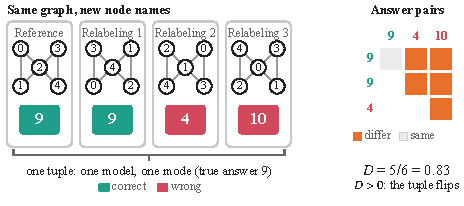
\includegraphics[width=\columnwidth]{figures/fig1_tuple.pdf}
\caption{One tuple: Qwen3-8B answering Erdős triangles-0000 directly under four labelings of one graph (drawn schematically). Green answers are correct, red wrong. Five of the six answer pairs differ, so $D = 0.83$.}
\label{fig:1}
\end{figure}

\textbf{Correctness:} An answer is correct when it equals the true answer. When a question has several correct answers, for example two equally short paths, any of them is correct. Density and diameter on Erdős are real numbers, so there we accept an answer within 0.01 of the true value (1\% for values above 1), so that a density written as 0.27 instead of 0.2727 counts. A crash, a timeout or an unreadable reply counts as wrong.

\textbf{Performance:} Accuracy is the share of all answers that are correct. Robust accuracy is the share of tuples in which every answer is correct.

\textbf{Invariance:} A tuple \emph{flips} when at least one of its answers differs from the others. When a question has several correct answers, they count as the same answer, and a missing answer counts as an answer of its own. The flip rate is the share of tuples that flip. Crossing flips with correctness divides the tuples into six buckets (Table 1): (1) the same correct answer on every serialization, (2) the same wrong answer on every serialization, (3) different answers that are all correct, (4) a flip with every serialization answered, (5) a flip in which some serializations gave no answer, and (6) no answer on any serialization. Buckets 4 and 5 are the flips. Bucket 2 holds errors that invariance cannot see, since a tuple can be stable and wrong.

\textbf{Weighted flips:} The flip rate treats every flip alike, whether one answer deviates or all of them differ. We therefore define two measures on a tuple with answers $a_1, \ldots, a_n$ and true answer $y$. $D$ is the fraction of answer pairs that differ, and $S$ is the range of the answers relative to the true answer:
\begin{gather*}
D = \frac{1}{\binom{n}{2}} \sum_{1 \le i < j \le n} \mathds{1}\left[a_i \neq a_j\right], \\
S = \frac{\max_{i} a_i - \min_{i} a_i}{|y|}
\end{gather*}

Here $\mathds{1}[\cdot]$ is 1 when its condition holds and 0 otherwise. $D$ is 0 when all answers agree and 1 when all differ: (1, 2, 2, 2) has $D = 0.5$ and (1, 2, 3, 4) has $D = 1$. $S$ applies to numeric answers, and $S = 1$ means the answers span the whole true value, as when a count doubles. $S$ uses only the answers that exist and divides by 1 when $y = 0$. The mean of $D$ over flipped tuples is the \emph{severity} of the flips.

\textbf{Localization:} Three measures locate where code breaks. (a) Each failed M2 answer is assigned the first step that failed: copy (a transcription error in the sense of Section 3.4), solve (a logic error: the right graph but a wrong answer) or run (an execution failure: a crash or timeout). (b) Each flipped M2 tuple is assigned where its serializations diverge: copy (one serialization declared a wrong graph), crash (one gave no answer) or program (every copy was right and every program ran, yet the answers differ). (c) The flip rates of M2 and M3 are compared on the same tuples, under relabeling and order only.

\textbf{Statistics:} A share is computed over the tuples (or answers) of one dataset, mode and factor, with the four models counting equally. We report GraphQA and Erdős separately and never average them together, since their tasks differ. To compare two modes on the same tuples we use McNemar's exact test for flips and the Wilcoxon signed-rank test for $D$, run for each model, dataset and library and Holm-corrected over the 16 cases. A logistic regression of flipping on mode, factor, model and task gives odds ratios, with errors clustered by graph. Intervals are 95\% bootstrap intervals over graphs. Finally, we ask identical prompts again and report how often the answer changes, as a floor for the flip rate.

\section{Results and Discussion}

We ask whether executed code returns the same answer when the same graph is serialized differently and, when it does not, where the fragility enters.

\subsection{Does executed code keep its answer, and more often than direct answering?}

Executed code flips far less often than direct answering, but is still not invariant. Under relabeling and edge order, direct answers (M1) flip on 11.9\% of GraphQA tuples and 20.8\% of Erdős tuples. Code from text (M2) flips on 4.8\% and 3.5\% in plain Python and on 6.8\% and 4.5\% with NetworkX. The gap between direct answering and plain-Python code is 5.7–8.6 points on GraphQA and 16.0–18.7 points on Erdős (95\% intervals), and code flips significantly less in 14 of 16 model $\times$ dataset $\times$ library cells. Both exceptions are Gemma 4 31B on GraphQA, whose direct answers are already the most stable (3.0\%). With model, task and factor held fixed, plain-Python code has 0.27 times the odds of a flip [0.25, 0.30] and NetworkX code 0.37 [0.34, 0.42].

\begin{figure}[t]
\centering
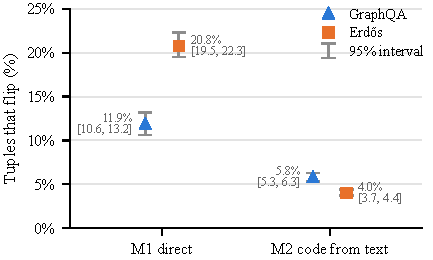
\includegraphics[width=\columnwidth]{figures/fig2_flip_by_mode.pdf}
\caption{Flip rate of direct answering (M1) and code from text (M2) under relabeling and edge order. M2 is averaged over plain Python and NetworkX. Whiskers are 95\% confidence intervals over the choice of graphs: we resample the graphs of each dataset with replacement 2,000 times and recompute the rate.}
\label{fig:2}
\end{figure}

On Erdős, code's flips are also milder. Four in five plain-Python flips have a single serialization out of line ($D = 0.5$), against two in five for direct answering, and a fifth of direct flips give four different answers. Severity is 0.54 against 0.71, so weighting by $D$ widens the gap from 6$\times$ to 8$\times$. On GraphQA severity barely differs (0.56 against 0.62).

\begin{figure}[t]
\centering
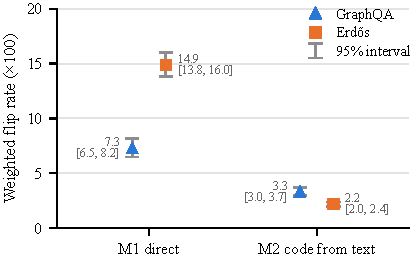
\includegraphics[width=\columnwidth]{figures/fig3_weighted_by_mode.pdf}
\caption{Weighted flip rate (mean $D$ over all tuples) of M1 and M2 under relabeling and edge order. M2 is averaged over plain Python and NetworkX. Whiskers are 95\% confidence intervals over the choice of graphs, computed as in Figure 2.}
\label{fig:3}
\end{figure}

The gap grows with the graph (Figure 4). Direct answering flips more with every step up in graph size and is worst on the largest graphs: from 7.7\% to 23.1\% of tuples on GraphQA and from 6.1\% to 36.2\% on Erdős, between graphs with up to 10 edges and graphs with more than 40. Code stays between 1.5\% and 8.2\% throughout. With task and model held fixed, each doubling of the edge count multiplies direct answering's odds of a flip by 2.06 [1.91, 2.22] and plain-Python code's by 1.19 [1.08, 1.31]. Within single tasks, direct answering flips more on the largest third of graphs than on the smallest in 16 of 19 tasks.

\begin{figure}[t]
\centering
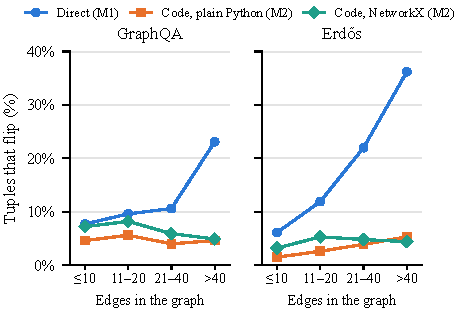
\includegraphics[width=\columnwidth]{figures/fig4_graph_size.pdf}
\caption{Share of tuples that flip under relabeling and edge order, by the number of edges, four models pooled.}
\label{fig:4}
\end{figure}

Part of every flip rate is resampling noise. Asked the identical prompt again, Qwen3-8B's code exceeds that floor in all 8 cells, by 5.0–12.6 points, while the other three models' code does so in only 7 of 24, so their small residual is close to noise.

A stable answer is not always a correct one (Table 1). On GraphQA, 8.1\% of plain-Python tuples give the same wrong answer on every serialization, mostly on two node-set questions that the DeepSeek models read the same wrong way. Invariance cannot see these errors, so we report robust accuracy beside it: 87.2\% of GraphQA and 95.9\% of Erdős plain-Python tuples are correct on every serialization, against 76.7\% and 78.6\% for direct answering.

\begin{table}[t]
\centering
\small\setlength{\tabcolsep}{3.2pt}
\begin{tabular}{@{}lrrrrrr@{}}
\toprule
 & \multicolumn{3}{c}{GraphQA} & \multicolumn{3}{c}{Erd\H{o}s} \\
\cmidrule(lr){2-4} \cmidrule(l){5-7}
Bucket & Dir. & Py & NX & Dir. & Py & NX \\
\midrule
(1) Same, correct & 76.7 & 87.2 & 85.4 & 74.9 & 91.3 & 85.8 \\
(2) Same, wrong & 11.4 & 8.1 & 7.7 & 0.5 & 0.6 & 0.3 \\
(3) Different, all correct & 0.0 & 0.0 & 0.0 & 3.8 & 4.5 & 4.3 \\
(4) Flip, all answered & 11.5 & 4.7 & 5.5 & 17.6 & 2.7 & 0.9 \\
(5) Flip with a crash & 0.3 & 0.0 & 1.2 & 3.2 & 0.9 & 3.6 \\
(6) No answer on all & 0.0 & 0.0 & 0.1 & 0.0 & 0.0 & 5.0 \\
\bottomrule
\end{tabular}
\caption{Tuples by bucket under relabeling and edge order, \% of tuples, four models pooled. Buckets 4 and 5 are the flips. Dir. = M1. Py and NX = M2 in plain Python and with NetworkX.}
\label{tab:1}
\end{table}

\subsection{Which factor flips the answer?}

Edge structure flips plain-Python answers the most, and NetworkX-code syntax flips NetworkX answers by crashing the programs. Relabeling and order permute the same text, and code barely reacts to them: 3.5–7.2\% of code tuples flip. Structure and syntax encode the graph differently, and each breaks one library (Table 2). With model and task held fixed, structure raises the odds of a flip 1.85-fold relative to relabeling [1.73, 1.96], and syntax 1.43-fold [1.35, 1.52].

\begin{table}[t]
\centering
\small\setlength{\tabcolsep}{3.2pt}
\begin{tabular}{@{}lrrrrrr@{}}
\toprule
 & \multicolumn{3}{c}{GraphQA} & \multicolumn{3}{c}{Erd\H{o}s} \\
\cmidrule(lr){2-4} \cmidrule(l){5-7}
Factor & Dir. & Py & NX & Dir. & Py & NX \\
\midrule
Relabeling & \textbf{12.6} & 5.6 & 7.2$^\dagger$ & \textbf{22.1} & 3.6 & 4.7 \\
Order & \textbf{11.1} & 4.0 & 6.3$^\dagger$ & \textbf{19.6} & 3.5 & 4.3 \\
Structure & \textbf{19.2} & \textbf{18.5}$^\dagger$ & 8.0 & \textbf{19.5} & \textbf{13.7} & \textbf{10.2} \\
Syntax & \textbf{14.9} & 4.8 & \textbf{13.6}$^\dagger$ & \textbf{18.9} & 3.8 & \textbf{16.6}$^\dagger$ \\
\bottomrule
\end{tabular}
\caption{Flip rate by factor, \% of tuples, four models pooled. Executed code keeps its answer far more often than direct answering, except under edge structure (Py) and NetworkX-code syntax (NX). Bold: 10\% or more. $^\dagger$: some model's code flips at least 1 point more often than its own direct answers. Dir. = M1. Py and NX = M2 in plain Python and with NetworkX.}
\label{tab:2}
\end{table}

\textbf{Structure:} Listing each undirected edge in both directions makes plain-Python programs count it twice, and 18.5\% of GraphQA and 13.7\% of Erdős tuples flip. On GraphQA node degree, 176 of Qwen3-8B's 200 answers are exactly double the true degree (DeepSeek-V3.1 147, DeepSeek-V4-Flash 51, Gemma 0). These flips are far off, not just different. Their median spread $S$ is 1.0 on both datasets, and 93\% (GraphQA) and 47\% (Erdős) contain an exact doubling. A NetworkX \texttt{Graph} merges the duplicates, so NetworkX code flips less (8.0\% and 10.2\%). Accuracy follows: structure costs plain-Python code 9.8 points on GraphQA and 6.7 on Erdős, while relabeling and order cost code at most 0.7.

\textbf{Syntax:} When the graph arrives as NetworkX code, NetworkX programs crash on some serializations and not on others, and 13.6\% and 16.6\% of tuples flip. Qwen3-8B's programs leave out the import, and DeepSeek-V4-Flash's use a \texttt{G} they never define. This serialization is itself code, so the effect exists only in code-writing modes. It costs NetworkX code 6.2 points of accuracy on Erdős, while plain-Python code is unaffected (4.8\% and 3.8\% flip).

\subsection{Which failures accompany a flip?}

Most flips start in the program the model writes, and few in its copy of the graph. The graph a program declares matches the input in 98.1–99.9\% of code answers. Among failed plain-Python answers, the solving step accounts for 97.5–99\% on GraphQA and 77–81\% on Erdős, while with NetworkX crashes account for 65–98\% of Erdős failures. A wrong copy is at most about 10\% of failures, and it does not reveal itself: 64\% (GraphQA) and 60\% (Erdős) of programs that declare a wrong graph still answer correctly.

Failures are not flips, though. On GraphQA the same wrong answer on every serialization (8.1\% of plain-Python tuples) is more common than a flip (4.8\%). Figure 5 therefore attributes each flip itself to where its serializations diverge. On GraphQA, 95.5\% of plain-Python flips start in the program. On Erdős the program still leads (61.5\%), but a crash starts 20.9\%, mostly DeepSeek-V4-Flash's, and a wrong copy 17.6\%: 35 of DeepSeek-V3.1's 40 flips come from a wrong copy of a long edge list.

\begin{figure}[t]
\centering
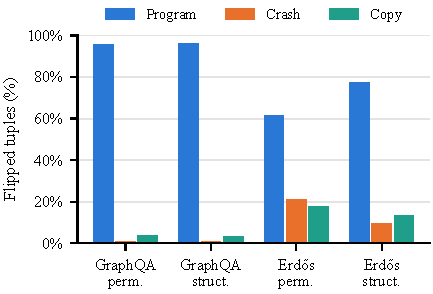
\includegraphics[width=\columnwidth]{figures/fig5_where_flips_start.pdf}
\caption{Where plain-Python flips start, four models pooled.}
\label{fig:5}
\end{figure}

The M3 control points the same way. Under edge order, Graph-as-Code runs one program on every ordering and flips on 0.0–0.1\% of tuples, against 3.5–6.3\% for M2, so a fixed program does not care about the order. M2 flips significantly more than M3 in 11 of 16 cells. The comparison is a diagnostic, not a causal estimate, since M3 also hides the graph from the model.

The rewritten program usually answers a different, coherent question (Figure 6). On the two node-list questions, 76\% of code flips (368 of 485) contain exactly the other reading's answer: every reachable node instead of the neighbours, or the reverse. On Erdős neighbors, all 76 of Qwen3-8B's flips contain a strict subset of the true neighbours, as a directed reading of the graph would.

\begin{figure}[t]
\centering
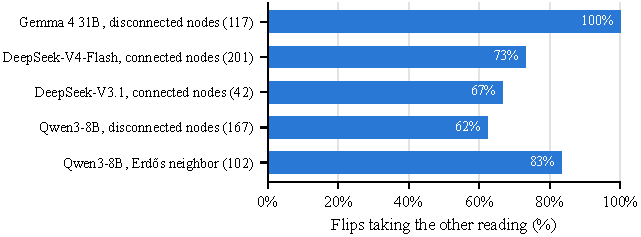
\includegraphics[width=\columnwidth]{figures/fig6_other_reading.pdf}
\caption{Share of code flips that contain the answer to the other reading of the question.}
\label{fig:6}
\end{figure}

Finally, serialization includes what is \emph{not} written. Our injected-data control omitted the word ``undirected'' from the Erdős prompt. Where the preamble asserts the graph is undirected, no program built a directed graph, and where it says nothing only one did; where it names ``directed'' only to define a conditional that does not apply, \emph{all four models} built a directed graph on every undirected instance they could be observed on, and every arm scored 28/100. Stating the type gives 100/100. The error is also partly invisible: 12 of the 84 undirected answers were still correct, and where the preamble describes both cases Gemma built a directed graph for 69\% of recovered graphs, nearly three quarters still correct.

\subsection{What the sensitivity is good for}

The instability is also a signal. Flagging an instance when its answers disagree across permutations catches most silent errors where the errors vary with the serialization: 73–94\% for Qwen3-8B and Gemma on GraphQA and for Qwen3-8B's Erdős plain Python, at flag rates of 5–17\%. It cannot see an error that stays the same. Both DeepSeek models misread \texttt{disconnected\_nodes} identically under every serialization, and none of those errors is caught. Detection finds unstable readings, not stable misreadings. Appendix C gives the detector per model and the mitigations we tried.

\subsection{Keeping the graph out of the prompt}

The most direct way to avoid the sensitivity is not to show the model the serialization at all. In Graph-as-Code (M3) the model writes its program from the task and the question alone, and the graph reaches the program as data. Structure and syntax therefore never reach the model, and relabeling and order change its prompt only when the question names a node. This costs no accuracy: with plain Python, M3 is the most accurate mode on both datasets (Table 3). It answers 92.9\% of GraphQA and 97.5\% of Erdős questions correctly, against 88.3\% and 96.9\% for code from text and 84.4\% and 87.0\% for direct answering, and it is correct on every serialization in 92.2\% and 97.3\% of tuples, against 87.2\% and 95.9\% for code from text.

\begin{table}[t]
\centering
\small\setlength{\tabcolsep}{4pt}
\begin{tabular}{@{}lrrrrr@{}}
\toprule
 & M1 & \multicolumn{2}{c}{M2} & \multicolumn{2}{c}{M3} \\
\cmidrule(lr){3-4} \cmidrule(l){5-6}
 &  & Py & NX & Py & NX \\
\midrule
\multicolumn{6}{@{}l}{\emph{Accuracy, all serializations}} \\
GraphQA & 84.4 & 88.3 & 88.8 & \textbf{92.9} & 87.0 \\
Erdős & 87.0 & 96.9 & 91.1 & \textbf{97.5} & 89.1 \\
\addlinespace
\multicolumn{6}{@{}l}{\emph{Robust accuracy, relabeling and order}} \\
GraphQA & 76.7 & 87.2 & 85.4 & \textbf{92.2} & 86.8 \\
Erdős & 78.6 & 95.9 & 90.2 & \textbf{97.3} & 89.0 \\
\bottomrule
\end{tabular}
\caption{Accuracy of every mode, \% of answers (upper panel) and of tuples correct on every serialization (lower panel), four models pooled. M3 receives no graph in its prompt; on Erdős its prompt states the graph type (see text). Bold: highest in the row. Py and NX = plain Python and NetworkX.}
\label{tab:3}
\end{table}

Without the graph text, the prompt itself must say whether the graph is directed. GraphQA's M3 prompts do, but our first M3 run on Erdős left it to each task's own instructions. On \texttt{neighbor} these mention only the directed case (``For directed graph, you should return the successors of the node''), so every model built a directed graph and answered 28 of 100 instances correctly (Section 5.3). Code from text sees the edge list and is not misled. We therefore added one sentence to every undirected M3 prompt, ``The graph is undirected: (u, v) and (v, u) denote the same edge.'', and reran M3 on Erdős; Table 3 reports this run. The sentence raises \texttt{neighbor} to 100 of 100 for every model and library, and also fixes two single-model misreadings, DeepSeek-V3.1's \texttt{has\_cycle} and Gemma's \texttt{edge\_existence}. Because every M3 program was generated afresh, a few tasks answered by a single program moved by chance in both directions (for example \texttt{bridges}). Appendix E gives the first run, in which plain-Python M3 is 5.7 points below code from text on Erdős.

Two limits remain. With NetworkX, M3 stays about 2 points below code from text in accuracy. And M3's errors are systematic: when the question names no node, one program answers every instance of a task, so a wrong program is wrong on every graph and every serialization, and disagreement across serializations (Section 5.4) cannot flag it.

\section{Conclusion and Limitations}

Executed code is more robust than direct answering to relabeling and edge order for most models, but it is not invariant, and not under every factor: listing each edge in both directions, or writing the graph as NetworkX code, brings code close to direct answering. The fragility does not enter where expected. Graphs are transcribed almost perfectly, and the failures sit in the solving code.

What remains of the sensitivity is partly usable. Permutation disagreement detects unstable errors at several calls per instance, and abstaining on it is nearly always right where they occur. It is partly beyond these levers: a model that misreads the question repeats that mistake under every serialization.

We are limited to four models on one gateway, small graphs (5–20 and 4–34 nodes) and zero-shot prompts where NetworkX is permitted, not required. Every experiment but the repeat baseline uses one generation per prompt, the deduplication hint covers two models, our pre-registered detection and per-task-solver targets are not met, and the canonical-labeling one only for two models. Where a question names no node, one shared M3 program can decide a task.

\bibliography{references}

\appendix
\counterwithin*{figure}{section}
\counterwithin*{table}{section}
\renewcommand{\thefigure}{\thesection\arabic{figure}}
\renewcommand{\thetable}{\thesection\arabic{table}}

\section{Prompt Examples}

Figure A1 shows the exact prompts of the three interaction modes for one GraphQA instance.

\begin{figure*}[p]
\small
\textbf{M1 (direct answering)}\par\smallskip
\begin{lstlisting}
In an undirected graph, (i,j) means that node i and node j are connected with an undirected edge. G describes a graph among nodes 0, 1, 2, 3, and 4.
The edges in G are: (1, 2) (1, 4) (2, 3).

Question: What is the degree of node 3?

Your answer should be an integer.

Solve the above problem efficiently and clearly. The last line of your response should be of the following format: 'Therefore, the final answer is: $\boxed{ANSWER}$.'
\end{lstlisting}
\textbf{M2 (code from text), plain-Python arm}\par\smallskip
\begin{lstlisting}
For this task, please calculate the degree of a given node in the undirected graph G.
Write a piece of Python code to return the answer in a variable 'ans'. Please enclose the code with # CODE START and # CODE END.

Fill in the template below and keep its structure. 'nodes' must list every node of G and 'edges' must list every edge of G as (u, v) pairs. Then write the code that computes the answer from 'nodes' and 'edges'. Compute the result - do not write it directly.

# CODE START
nodes = <the nodes of G>
edges = <the edges of G, as (u, v) pairs>

<your code here>
ans = <the computed result, a Python int>
# CODE END

Use only plain Python and its standard library. Do not import networkx or any other third-party library.

Q: What is the degree of node 3?
In an undirected graph, (i,j) means that node i and node j are connected with an undirected edge. G describes a graph among nodes 0, 1, 2, 3, and 4.
The edges in G are: (1, 2) (1, 4) (2, 3).
A:
\end{lstlisting}
\textbf{M3 (Graph-as-Code), plain-Python arm: the parts that differ from M2}\par\smallskip
\begin{lstlisting}
[... first two lines as in M2 ...]

Fill in the template below and keep its structure. The variables 'nodes' (the nodes of G) and 'edges' (the edges of G, as (u, v) pairs) are already defined; use them directly and do not redefine them. Compute the result - do not write it directly.

# CODE START
# 'nodes' and 'edges' are already defined.

<your code here>
ans = <the computed result, a Python int>
# CODE END

[... library line as in M2 ...]

Q: What is the degree of node 3?
A:
\end{lstlisting}
Defined by the harness before the M3 program runs:\par\smallskip
\begin{lstlisting}
nodes = [0, 1, 2, 3, 4]
edges = [(1, 2), (1, 4), (2, 3)]
\end{lstlisting}
\caption{The prompts for one GraphQA instance, a 5-node graph with the question ``What is the degree of node 3?'' (answer 1), in the plain-Python arm. M1 uses the system prompt ``You are a helpful assistant.''; M2 and M3 use one describing an expert in graph networks and Python. In the NetworkX arm, the library line reads ``You may use the networkx library.''}
\label{fig:A1}
\end{figure*}

\section{Per-model Results}

Figures B1 and B2 and Tables B1 and B2 repeat Figures 2 and 3 and Tables 1 and 2 for each model instead of pooling the four. On Erdős every model's code flips less than its direct answers. On GraphQA the exception is Gemma 4 31B, whose direct answers are the most stable of all (3.0\%) and whose code flips on 4.3\%. Qwen3-8B flips most in every mode and dataset.

\begin{figure*}[t]
\centering
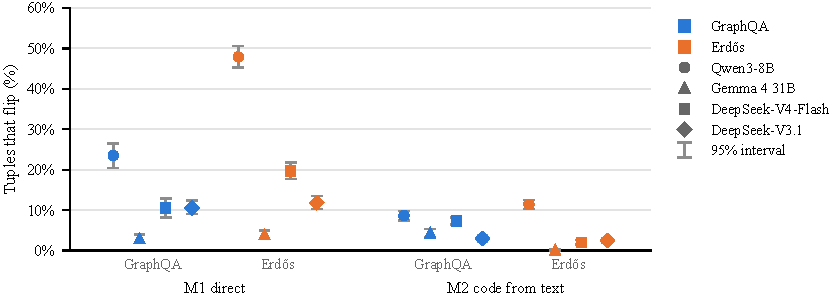
\includegraphics[width=0.9\textwidth]{figures/figB1_flip_by_model.pdf}
\caption{Flip rate of M1 and M2 for each model under relabeling and edge order, as in Figure 2 but without pooling the models. Color marks the dataset and shape the model. M2 is averaged over plain Python and NetworkX. Whiskers are 95\% confidence intervals over the choice of graphs, computed as in Figure 2.}
\label{fig:B1}
\end{figure*}

\begin{figure*}[t]
\centering
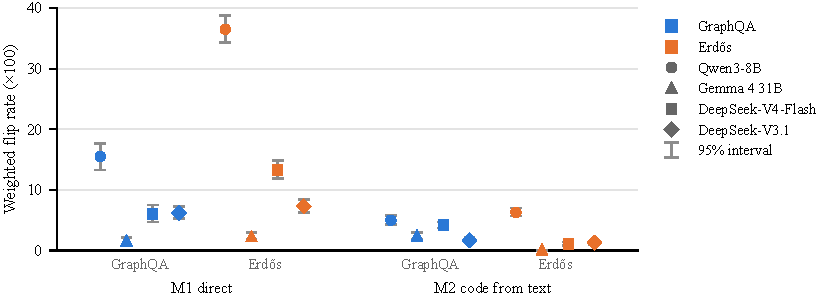
\includegraphics[width=0.9\textwidth]{figures/figB2_weighted_by_model.pdf}
\caption{Weighted flip rate (mean $D$ over all tuples) for each model under relabeling and edge order, as in Figure 3. Whiskers as in Figure B1.}
\label{fig:B2}
\end{figure*}

\begin{table}[t]
\centering
\small\setlength{\tabcolsep}{3.2pt}
\begin{tabular}{@{}lrrrrrr@{}}
\toprule
 & \multicolumn{3}{c}{GraphQA} & \multicolumn{3}{c}{Erd\H{o}s} \\
\cmidrule(lr){2-4} \cmidrule(l){5-7}
Bucket & Dir. & Py & NX & Dir. & Py & NX \\
\midrule
\multicolumn{7}{@{}l}{\emph{Qwen3-8B}} \\
(1) Same, correct & 69.8 & 93.8 & 84.5 & 48.5 & 84.6 & 60.7 \\
(2) Same, wrong & 6.6 & 0.4 & 3.7 & 1.0 & 1.8 & 0.9 \\
(3) Different, all correct & 0.0 & 0.0 & 0.0 & 2.6 & 4.8 & 4.5 \\
(4) Flip, all answered & 22.2 & 5.6 & 9.1 & 42.4 & 7.8 & 1.2 \\
(5) Flip with a crash & 1.2 & 0.1 & 2.3 & 5.5 & 1.0 & 12.8 \\
(6) No answer on all & 0.1 & 0.0 & 0.4 & 0.0 & 0.0 & 20.0 \\
\addlinespace
\multicolumn{7}{@{}l}{\emph{Gemma 4 31B}} \\
(1) Same, correct & 87.5 & 95.3 & 94.6 & 92.2 & 95.5 & 95.6 \\
(2) Same, wrong & 9.5 & 1.0 & 0.5 & 0.1 & 0.0 & 0.0 \\
(3) Different, all correct & 0.0 & 0.0 & 0.0 & 3.7 & 4.4 & 4.2 \\
(4) Flip, all answered & 3.0 & 3.7 & 4.8 & 3.4 & 0.1 & 0.0 \\
(5) Flip with a crash & 0.0 & 0.0 & 0.1 & 0.6 & 0.1 & 0.1 \\
(6) No answer on all & 0.0 & 0.0 & 0.0 & 0.0 & 0.0 & 0.0 \\
\addlinespace
\multicolumn{7}{@{}l}{\emph{DeepSeek-V4-Flash}} \\
(1) Same, correct & 75.7 & 74.9 & 78.6 & 75.3 & 91.5 & 94.8 \\
(2) Same, wrong & 13.8 & 18.0 & 13.9 & 0.7 & 0.6 & 0.4 \\
(3) Different, all correct & 0.0 & 0.0 & 0.0 & 4.3 & 4.4 & 4.2 \\
(4) Flip, all answered & 10.5 & 7.1 & 7.5 & 17.9 & 1.3 & 0.6 \\
(5) Flip with a crash & 0.0 & 0.0 & 0.0 & 1.8 & 2.2 & 0.0 \\
(6) No answer on all & 0.0 & 0.0 & 0.0 & 0.0 & 0.0 & 0.0 \\
\addlinespace
\multicolumn{7}{@{}l}{\emph{DeepSeek-V3.1}} \\
(1) Same, correct & 73.7 & 84.6 & 83.9 & 83.5 & 93.8 & 92.3 \\
(2) Same, wrong & 15.8 & 12.8 & 12.7 & 0.2 & 0.0 & 0.0 \\
(3) Different, all correct & 0.0 & 0.0 & 0.0 & 4.4 & 4.6 & 4.4 \\
(4) Flip, all answered & 10.4 & 2.6 & 0.9 & 6.9 & 1.5 & 2.0 \\
(5) Flip with a crash & 0.1 & 0.0 & 2.4 & 4.9 & 0.1 & 1.3 \\
(6) No answer on all & 0.0 & 0.0 & 0.1 & 0.0 & 0.0 & 0.0 \\
\bottomrule
\end{tabular}
\caption{Tuples by bucket for each model under relabeling and edge order, as in Table 1 (\% of tuples). Dir. = M1. Py and NX = M2 in plain Python and with NetworkX.}
\label{tab:B1}
\end{table}

\begin{table}[t]
\centering
\small\setlength{\tabcolsep}{3.2pt}
\begin{tabular}{@{}lrrrrrr@{}}
\toprule
 & \multicolumn{3}{c}{GraphQA} & \multicolumn{3}{c}{Erd\H{o}s} \\
\cmidrule(lr){2-4} \cmidrule(l){5-7}
Factor & Dir. & Py & NX & Dir. & Py & NX \\
\midrule
\multicolumn{7}{@{}l}{\emph{Qwen3-8B}} \\
Relabeling & \textbf{24.3} & 7.3 & \textbf{12.7} & \textbf{49.2} & 8.9 & \textbf{14.4} \\
Order & \textbf{22.6} & 4.2 & \textbf{10.0} & \textbf{46.7} & 8.8 & \textbf{13.6} \\
Structure & \textbf{32.0} & \textbf{40.3$^\dagger$} & \textbf{18.7} & \textbf{49.5} & \textbf{35.1} & \textbf{28.5} \\
Syntax & \textbf{27.4} & 4.9 & \textbf{39.3$^\dagger$} & \textbf{49.1} & 9.9 & \textbf{34.2} \\
\addlinespace
\multicolumn{7}{@{}l}{\emph{Gemma 4 31B}} \\
Relabeling & 3.3 & 4.1 & 5.6$^\dagger$ & 4.3 & 0.2 & 0.2 \\
Order & 2.8 & 3.2 & 4.2$^\dagger$ & 3.6 & 0.2 & 0.0 \\
Structure & 9.3 & 2.7 & 3.1 & 3.3 & 0.9 & 1.4 \\
Syntax & 6.9 & 3.6 & 4.3 & 2.6 & 0.4 & 0.8 \\
\addlinespace
\multicolumn{7}{@{}l}{\emph{DeepSeek-V4-Flash}} \\
Relabeling & \textbf{11.9} & 7.9 & 7.3 & \textbf{21.9} & 3.4 & 0.6 \\
Order & 9.1 & 6.2 & 7.7 & \textbf{17.4} & 3.6 & 0.6 \\
Structure & \textbf{16.9} & \textbf{17.0} & 7.3 & \textbf{15.8} & \textbf{11.4} & 7.8 \\
Syntax & \textbf{13.3} & 7.6 & 6.7 & \textbf{15.8} & 4.3 & \textbf{29.7$^\dagger$} \\
\addlinespace
\multicolumn{7}{@{}l}{\emph{DeepSeek-V3.1}} \\
Relabeling & \textbf{11.0} & 3.0 & 3.3 & \textbf{13.0} & 1.8 & 3.4 \\
Order & \textbf{10.0} & 2.2 & 3.3 & \textbf{10.7} & 1.5 & 3.2 \\
Structure & \textbf{18.7} & \textbf{14.0} & 2.9 & 9.4 & 7.4 & 3.1 \\
Syntax & \textbf{12.0} & 3.3 & 4.1 & 8.2 & 0.7 & 1.6 \\
\bottomrule
\end{tabular}
\caption{Flip rate by factor for each model, as in Table 2 (\% of tuples). Bold: 10\% or more. $^\dagger$: the model's code flips at least 1 point more often than its own direct answers.}
\label{tab:B2}
\end{table}

Here \emph{I} is the share of tuples whose serializations all return literally the same answer, and \emph{R} the share where every serialization is correct.

\begin{table*}[t]
\centering
\small
\begin{tabular}{@{}ll*{6}{>{\centering\arraybackslash}p{2.4em}}@{}}
\toprule
 &  & \multicolumn{2}{c}{Direct} & \multicolumn{2}{c}{Native} & \multicolumn{2}{c}{NetworkX} \\
\cmidrule(lr){3-4} \cmidrule(lr){5-6} \cmidrule(l){7-8}
Dataset & Model & I & R & I & R & I & R \\
\midrule
GraphQA & Qwen3-8B & 76 & 70 & 94 & 94 & 88 & 85 \\
GraphQA & Gemma 4 31B & 97 & 87 & 96 & 95 & 95 & 95 \\
GraphQA & DeepSeek-V4-F & 90 & 76 & 93 & 75 & 92 & 79 \\
GraphQA & DeepSeek-V3.1 & 89 & 74 & 97 & 85 & 97 & 84 \\
Erdős & Qwen3-8B & 50 & 51 & 86 & 89 & 62 & 65 \\
Erdős & Gemma 4 31B & 92 & 96 & 95 & 100 & 96 & 100 \\
Erdős & DeepSeek-V4-F & 76 & 80 & 92 & 96 & 95 & 99 \\
Erdős & DeepSeek-V3.1 & 84 & 88 & 94 & 98 & 92 & 97 \\
\bottomrule
\end{tabular}
\caption{Consistency I and correctness R on all serializations (\%), averaged over relabeling and edge order.}
\label{tab:B3}
\end{table*}

\section{Mitigation}

\begin{table}[t]
\centering
\small\setlength{\tabcolsep}{3.2pt}
\begin{tabular}{@{}llrrr@{}}
\toprule
Data & Model & Flag & Caught & Abst. (cov.) \\
\midrule
GraphQA & Qwen3-8B & 9.1 & 88.9 & 99.7 (90.9) \\
GraphQA & Gemma 4 31B & 5.1 & 75.0 & 99.4 (94.9) \\
GraphQA & DeepSeek-V4-F & 9.1 & 26.3 & 82.4 (90.9) \\
GraphQA & DeepSeek-V3.1 & 3.4 & 1.1 & 86.8 (96.6) \\
Erdős & Qwen3-8B & 17.1 & 72.7 & 98.5 (82.9) \\
Erdős & DeepSeek-V4-F & 9.5 & 53.8 & 99.4 (90.5) \\
Erdős & DeepSeek-V3.1 & 8.1 & 1 of 1 & 100 (91.9) \\
Erdős & Gemma 4 31B & 5.0 & — & 100 (95.0) \\
\bottomrule
\end{tabular}
\caption{Permutation disagreement as an error detector, plain-Python arm (\%). Caught: wrong answers that returned one (a crash needs no detector). Abst.: accuracy when answering only if all permutations agree (share answered).}
\label{tab:C1}
\end{table}

Where errors vary with the serialization it catches most of them: 73–94\% of silent errors for Qwen and Gemma on GraphQA (both arms) and Qwen's Erdős plain Python at 5–17\% flag rates, where abstaining answers 83–95\% of instances at 97.3–99.8\% accuracy, and 54–56\% on Erdős for DeepSeek-V4-Flash's plain Python and Qwen's crash-heavy NetworkX arm. For Qwen's GraphQA plain Python one extra relabeled call is enough: 15 of 18 errors at a 4.4\% flag rate.

The two cells where it fails are the result. Both DeepSeek models misread \texttt{disconnected\_nodes} identically under every serialization, and it holds 59–99\% of their GraphQA errors, none caught; Gemma makes the same misreading on only 16 graphs and 12 are caught. \emph{The blind spot is a property of the error, not of the model.} Detection finds unstable errors, not wrong beliefs.

Voting over the permuted answers moves code-arm accuracy by $-$2.4 to +6.4 points, and voting over the permuted programs, each run on one fixed graph, by $-$2.3 to +5.3 (on 300 instances per dataset): both help where errors are unstable and amplify a majority misreading where they are not. An exact canonical labeling renders every relabeling and reordering of every instance to one prompt; on a fixed-stride subset covering every task (400 GraphQA and 150 Erdős instances) it is significantly more accurate than random labels in 8 of 24 cells and less in one, on the ambiguous task. One solver per task, with no graph in the prompt, is free on Erdős for the three stronger models once told the graph type, but a single program decides a whole task: one misread task costs each of them 3–11 points in a GraphQA arm, and nonexistent NetworkX routines cost Qwen 4–7. A fixed adapter reconciles the prompt's two answer conventions, dropping a solver's own top-level call and returning an assigned but unreturned \texttt{ans}; it changes 17 Qwen programs and no others (Qwen's GraphQA plain-Python solver: 72\% without it). A one-sentence hint to count duplicate edges once, run later on two models against the original run on another machine (so provider drift is not excluded), coincides with duplicated-edge degree of 100 for DeepSeek-V3.1 (from 34 and 19) but 87 for Qwen, whose canonical degree falls from 99 to 86 and consistency under three unrelated factors by 6–13 points.

\section{Tuple Sizes}

\begin{table*}[t]
\centering
\small
\begin{tabular}{@{}p{0.11\textwidth}p{0.33\textwidth}p{0.22\textwidth}p{0.26\textwidth}@{}}
\toprule
Factor & Answers in a tuple & GraphQA & Erdős \\
\midrule
Relabeling & reference labeling + 3 random relabelings & 4 (699 tuples), 3 (1) & 4 (1,199), 3 (1) \\
Order & dataset's own order + 3 reorderings & 4 (587), 3 (63), 2 (39) & 4 (1,133), 3 (58), 2 (9) \\
Structure & reference + adjacency list + each edge in both directions & 3 (700) & 3 (1,123), 2 (77) \\
Syntax & reference + plain text, JSON, NetworkX code & 4 (700) & 3, JSON and NetworkX code only (1,200) \\
\bottomrule
\end{tabular}
\caption{Answers per tuple, with the number of tuples of each size per model and mode. A serialization identical to its reference is dropped, which shortens some tuples: 11 GraphQA instances have no order tuple, one random relabeling per dataset came out as the identity, and the 77 directed Erdős graphs have no both-directions serialization.}
\label{tab:D1}
\end{table*}

\section{M3 Without the Stated Graph Type}

Table E1 repeats Table 3 with the first M3 run on Erdős, whose prompts did not state that the graph is undirected (Section 5.5). Plain-Python M3 is then 5.7 points below code from text on Erdős, almost all of it on \texttt{neighbor}. The M3 control in Section 5.3 uses this first run.

\begin{table}[t]
\centering
\small\setlength{\tabcolsep}{4pt}
\begin{tabular}{@{}lrrrrr@{}}
\toprule
 & M1 & \multicolumn{2}{c}{M2} & \multicolumn{2}{c}{M3} \\
\cmidrule(lr){3-4} \cmidrule(l){5-6}
 &  & Py & NX & Py & NX \\
\midrule
\multicolumn{6}{@{}l}{\emph{Accuracy, all serializations}} \\
GraphQA & 84.4 & 88.3 & 88.8 & \textbf{92.9} & 87.0 \\
Erdős & 87.0 & \textbf{96.9} & 91.1 & 91.2 & 84.2 \\
\addlinespace
\multicolumn{6}{@{}l}{\emph{Robust accuracy, relabeling and order}} \\
GraphQA & 76.7 & 87.2 & 85.4 & \textbf{92.2} & 86.8 \\
Erdős & 78.6 & \textbf{95.9} & 90.2 & 91.0 & 84.1 \\
\bottomrule
\end{tabular}
\caption{Table 3 with the first M3 run on Erdős, before the graph type was stated in its prompt. M1, M2 and all of GraphQA are unchanged. Bold: highest in the row.}
\label{tab:E1}
\end{table}

\end{document}
